\documentclass[12pt,a4paper]{article}
\usepackage[utf8]{inputenc}
\usepackage{amsmath}
\usepackage{amsfonts}
\usepackage{amssymb}
\usepackage{graphicx}
\usepackage{pxfonts}
\usepackage{hyperref}
\usepackage{microtype}
\usepackage{a4wide}
\usepackage{multicol}
\usepackage{todonotes}
\usepackage{tabularx}
\usepackage{pdflscape}

% Capitalize 'Section 1.1'.
\renewcommand*{\sectionautorefname}{Section}
% Use 'Section 1.1' to refer to (sub)subsection 1.1.
\let\subsectionautorefname\sectionautorefname
\let\subsubsectionautorefname\sectionautorefname

\author{
\textbf{Group Mahler}\\~\\
  Van der Cruysse, Jonathan\\ \texttt{Jonathan.VanderCruysse@UGent.be}
  \and
  De Pontieu, Thomas\\ \texttt{Thomas.DePontieu@UGent.be}
  \and
 Weyns, Michael\\ \texttt{Michael.Weyns@UGent.be}
\and
Moreel, Sam\\ \texttt{Sam.Moreel@UGent.be}
\and
Vanlanduyt, Ignace\\ \texttt{Ignace.Vanlanduyt@UGent.be}
\and
Van Thienen, Philippe\\ \texttt{Philippe.VanThienen@UGent.be}
}
\title{A modest proposal for simple payments}
\begin{document}
	\maketitle
	
	\begin{abstract}
		This is a proposal for a payment system that is suitable for quick and convenient small to medium-sized transactions. The system's design is inspired by real-life checkbooks.
		
		The payment system's approach to tough problems such as the double-spending problem is not to make abuse entirely impossible but rather to make abuse unappealing to a rational actor by creating sufficient evidence to catch attackers red-handed.
	\end{abstract}

	\begin{multicols}{2}

	\section{Entities}
	\label{sec:entities}
	
	This section details the information managed by the various entities in the payment system, as well as the entities themselves.
	
	\paragraph{Account holders} An account holder is someone who can spend money using this payment system.
	
	\paragraph{The bank}
	
	An account holder's money is stored at the bank, which serves as a trusted third party. Money is never transferred directly between devices---the bank completes all transactions. Additionally, each bank has a unique public (stored on all account holder devices), private (stored only at the bank) key pair used for signing checks.
	
	\paragraph{Account holder devices}
	
	Each device registered for the payment system is associated with a particular bank account and has
	\begin{itemize}
		\item a unique public (stored at the bank), private (stored on the device) key pair,
		\item a monthly\footnote{Any other sufficiently large timespan would work just as well here, but monthly seems to be the conventional choice here.} spending cap (stored both on the device and at the bank), and
		\item a number of unspent checks, the \emph{checkbook} (stored on the device).
		\item an authentication certificate to authenticate the owner of the device.
	\end{itemize}

	It is worth clarifying that an account holder device is a \emph{logical} device that may, but does not have to, correspond to a physical device. For example, a phone that is authorized for $n$ different accounts acts as $n$ different account holder devices.

	\paragraph{Authentication certificate}
	
	Each Account holder device has an authentication certificate used to verify the identity of public key. The certificate contains
	\begin{itemize}
		\item the public key of the corresponding account holder device,
		\item an identification payload, usually the full name of the owner/store but this can also contain more complex data such as the coordinates of a store,
		\item an expiration date, after which this certificate should no longer be considered valid,
		\item a signiture over all previous fields by the bank,
		\item the bank id of issuing bank
	\end{itemize}


	\paragraph{Checks}
	
	Every check is unique and each check specifies
	
	\begin{itemize}
		\item a unique identifier for the bank that issued the check,
		\item the public key of the account holder device for which the check was issued,
		\item the check's value, that is, the maximum amount of money the check can be used for,
		\item a number that uniquely identifies the check within the space of all checks issued for the device; this can be a sequence number or a random number,
		\item an expiration date. Expired checks can no longer be used to make promissory notes, and
		\item a signature of the above produced by the private key of the bank that issued the check.
	\end{itemize}

	The number of checks is such that the total value of all checks on an account holder's device never exceeds the spending cap for that device.

	\paragraph{Promissory notes}
	
	A promissory note is an agreement between a ``buyer'' account holder and a ``seller'' account holder to transfer a particular amount of money from the former to the latter. Promissory notes are sent to the bank for processing. A fully signed promissory note consists of
	
	\begin{itemize}
		\item the seller's public key,
		\item a unique identifier (within the space of all promissory notes generated by this particular seller),
		\item the amount of money to transfer,
		\item a timestamp of the date on which the transaction between buyer and seller was made; promissory notes can only be claimed by the seller up to X days after the transaction date and checks can still be redeemed up to X days after they expired,
		\item a list of checks and the amount of money each check transfers (the total amount transferred by the checks equals the sum value on the promissory note),
		\item a signature of all aforementioned fields by the seller's private key, and
		\item a signature of all aforementioned fields by the buyer's private key.
	\end{itemize}

	A promissory note can be submitted to the bank, which will then wire the money from the buyer's account to the seller's. The creation and processing of promissory notes is described in more detail in \autoref{sec:protocols}.

	\section{Protocols}
	\label{sec:protocols}
	
	This section describes the protocols used to exchange information between actors.
	
	\subsection{Signing a promissory note}

	A promissory note is an agreement between two parties---a buyer and a seller---to transfer a particular amount of money from the buyer's account to the seller's. Promissory notes are redeemed by the seller when they can connect to their bank. From the buyer's perspective, signing a promissory note is the same as handing over cash to the seller. 
	
	This section describes the protocol for creating promissory notes.

	\subsubsection{Signing algorithm}
	
	The creation of a fully signed promissory note consists of a number of steps. The steps below are illustrated by \autoref{fig:signing_algorithm}.
	
	\begin{enumerate}
		\item The seller drafts a proto--promissory note that consists of the first fields of a promissory note: the seller's public key, a unique identifier for the promissory note and the amount of money to transfer.
		
		\item The seller sends the draft to the buyer.
		
		\item The buyer either chooses to agree to the transaction or not. If the buyer does not want to or cannot agree to the transaction, the seller's proto--promissory note is discarded.
		
		\item If the buyer agrees to the transaction, then they attach one or more checks to the proto--promissory note and tags each check with a particular amount of money to transfer. 
		
		\item This unsigned promissory note is sent back to the seller for signing.
		
		\item The seller signs the unsigned promissory note.
		
		\item The seller sends the resulting partially-signed promissory note to the buyer.
		
		\item The buyer signs the partially-signed promissory note, turning it into a fully-signed promissory note.
		
		\item This fully-signed promissory note is subsequently sent to the seller.
	\end{enumerate}

	After going through the motions described above, both the seller and the buyer retain a copy of the fully-signed promissory note, which doubles as a receipt.
	
	Anything short of a fully-signed promissory note is null and void---the bank will not accept, e.g., an unsigned or partially-signed promissory note.
	
	\end{multicols}
	\newpage
    
    \begin{landscape}
    \thispagestyle{empty}
    
    	\begin{figure}
        	\centering
    	    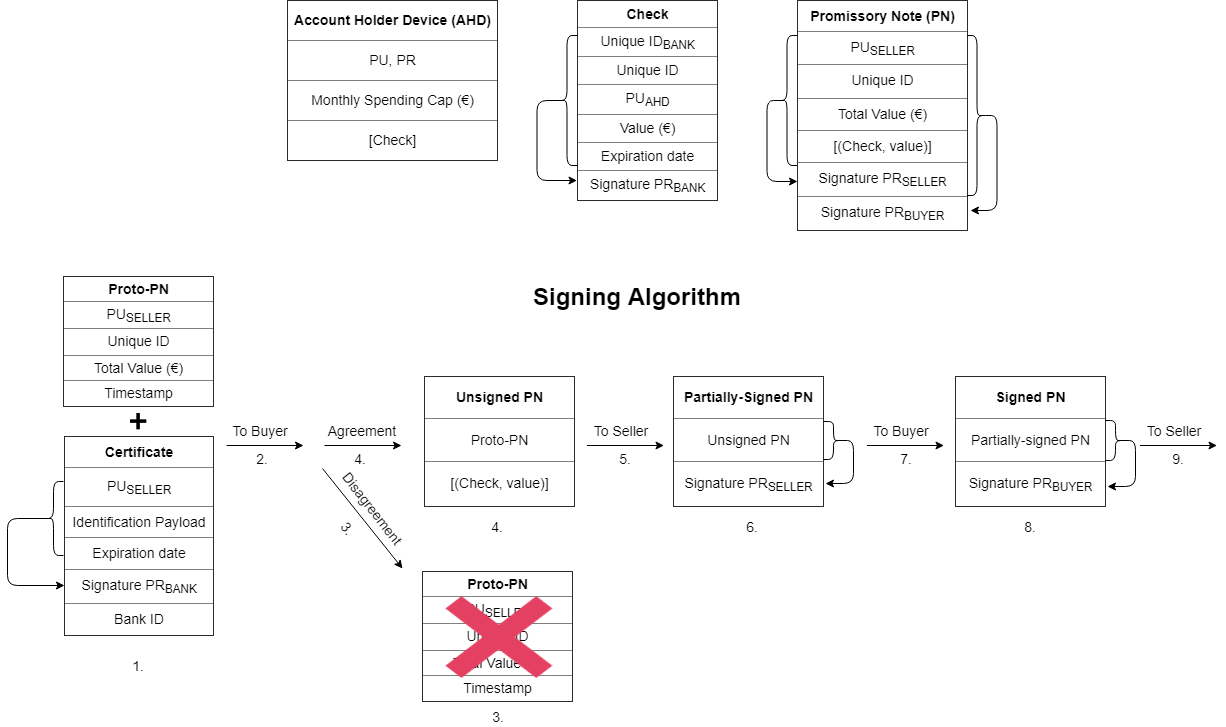
\includegraphics[width=503pt]{img/signing_algorithm}
            \caption{Signing Algorithm}
            \label{fig:signing_algorithm}
    	\end{figure}
        
        \vfill
		\raisebox{1em}{\makebox[\linewidth]{\thepage}}
    \end{landscape}
	
    \newpage
	\begin{multicols}{2}
	
	\subsubsection{Well-formedness}

	Implicit in the signing algorithm as described in the previous section is that the promissory note is well-formed:
	
	\begin{itemize}
		\item all signatures must be verified against their public keys by each party,
		\item the sum of the amounts of money specified by the checks must match the total amount on the promissory note, and
		\item the amount of money with which every check is tagged must not exceed the check's maximum value.
		\item the note should not contain checks that expired before the transaction date timestamp.
	\end{itemize}

	Additionally, each party should also make sure that the other party doesn't (subtly or otherwise) change the promissory note halfway through the transaction. For example, the seller should check that the amount of money specified by the unsigned promissory note sent to them by the buyer matches the amount the seller originally specified.
	
	It is also important for both parties to confirm the correctness of the timestamp, as an incorrect timestamp can result in the note being unredeemable by the seller (note expired before it can even be sent to the bank), or the note being redeemable beyond the intended expiration date.
	
	If the seller is online, then they must verify that the checks they receive have not been spent already. If they are offline, they cannot do so. See \autoref{sec:double-spending-checks} for a more thorough discussion of the double-spending problem.

	\subsubsection{Goals and security requirements}

	The promissory note signing algorithm achieves a number of security requirements.
	
	\paragraph{Data integrity}

	A fully-signed promissory note cannot be tampered with to, e.g., edit the amount of money transferred precisely because it is signed: both parties agreed to a particular document and nothing else.

	\paragraph{Non-repudiation}
	
	Both the seller and the buyer sign the promissory note with their private key, so neither party can claim that they did not assent to the transaction.
	
	\paragraph{Data-origin authentication}
	
	The origin of two components of a promissory note can be verified:
	
	\begin{itemize}
		\item the origin of the buyer's checks can be verified because they are signed by the bank that issued them---sellers are assumed to know the public keys of all banks that use the payment system---and
	
		\item the origin of the fully-signed promissory note can also be verified: it is signed by the buyer and contains the buyer's public key---this information is stored in the checks, which can be verified as per the previous bullet.
	\end{itemize}

	If the buyer can connect to their bank, then they can ask their bank if the seller is indeed an account holder, that is, they can verify the origin of the partially-signed promissory note before signing it themselves.
	
	If the buyer is offline, then they cannot verify the seller's authenticity. This lack of seller authentication is fairly harmless because a promissory note signed by a seller who is not also an account holder cannot be redeemed by the seller. This point is reiterated in \autoref{sec:lack-of-seller-authentication}.

	\subsubsection{Non-goals}

	The protocol described in this document aims to accomplish the goals stated in the previous section, but it consciously does not try to conform to the requirements listed in this section.

	The non-goals listed here are not considered entirely irrelevant to electronic payments. Rather, they are considered to be out of scope because a real-life implementation of the payment system is not intended to exist in isolation: there are already battle-tested solutions for the security requirements listed here and the payment system is envisioned to coexist with them instead of supplanting them.

	\paragraph{Data confidentiality}

	It is arguably desirable to prevent others from eavesdropping on a payment. The protocol described in this section does not address this directly. Confidentiality can be accomplished by running the protocol set out here over a secure channel, e.g., over TLS.

	\paragraph{Availability}

	After signing a promissory note, the seller should be able to submit the fully signed promissory note to the bank. Hence, one might argue that the bank's servers should be available whenever the seller has an Internet connection. However, the protocol with which an account holder communicates with their bank is left to the bank to specify, so any availability requirements it raises are out of scope.

	\subsection{Redeeming a promissory note as the seller}

	To redeem a promissory note, the seller sends it to their bank. The bank verifies the promissory note's authenticity and transfers the amount specified by the promissory note from the buyer's account to the seller's \emph{if this is the first time that the promissory note is redeemed.} Trying to redeem the same promissory note twice does nothing.
	
	Furthermore, promissory notes are no longer valid X days after the included timestamp. If a seller tries to redeem the note in this scenario, the debt is instead cleared from the buyer's account and, if applicable\footnote{See, Redeeming a promissory note as the buyer}, the buyer's monthly cap is restored to reflect the transaction now being declared void.

	The exact protocol used by the seller and the bank to redeem promissory notes is up to the bank to specify or implement. Similarly, the protocol used by banks to negotiate a wire transfer is not specified here either.

	It may be desirable to transfer promissory notes over a secure connection to prevent eavesdropping, but that is not necessary to make the payment system work. The signatures on a promissory note ensure that the note cannot be tampered with.
	
	\subsection{Redeeming a promissory note as the buyer}
	
	Buyers should be able to pass their fully signed promissory notes to their bank to confirm their successful transactions with the bank. This allows the bank to update the client's unspent checks and monthly spending cap in advance of the sellers redeeming the respective notes so that the client can request new checks with their bank. Without this option, if a buyer uses for example a \$500 check for a \$10 transaction, the buyer will be locked out of \$490 he can't spend until the seller redeems the promissory note with the bank.
	
	Additionally, checks have an expiration date that is tracked by the bank in case a seller never claims a promissory note and the buyer loses their copy of that same note. This extra measure prevents a buyer from being permanently locked out of spending parts of their money.
	
	A buyer passing a note to their bank should not necessarily trigger an actual money transfer as the burden of redeeming the note lies with the seller.

	\subsection{Transferring checks}

	At the start of each month\footnote{As stated before, the exact timespan doesn't really matter. A month is used here for simplicity.}, the bank signs a fresh batch of checks that have a total value equal to the account holder device's cap minus the total value of the user's.

	An account holder can send a request to the bank for these newly-generated checks.

	The protocol via which the account holder requests their new batch of checks and the bank transfers the checks is left up to the bank to specify as it is does not touch on the interaction between account holders.
	
	\section{Encodings}
	
	The entities described in \autoref{sec:entities} abstractly describe the information required to successfully run the payment system's protocols.
	
	To ensure compatibility between different implementations of the payment system, this section describes a file format for checks and promissory notes.
	
	Compatibility is to be understood in a narrow sense here: the objective is to ensure that promissory notes can be agreed upon and signed by users of different implementations. The communications between account holders and their banks are implementation-defined.
	
	\subsection{Data types}
	\label{sec:data-types}
	
	The encodings for checks and promissory notes make use of the following data types:
	
	\begin{itemize}
		\item \textbf{$k$-bit integers.} These are stored in little-endian byte order. Unless explicitly stated otherwise, all integers in this section are unsigned.
		
		\item \textbf{Length-prefixed strings.} A length-prefixed string consists of a 32-bit unsigned integer followed by $n$ bytes, where $n$ is the integer prefix.
		
		\item \textbf{Signatures.} A signature is a special kind of length-prefixed string. The contents of a signature are obtained by first taking the SHA3-256 hash of the data to which the signature pertains and then applying the FIPS 186-4 (EC)DSA algorithm to that hash \cite{fips-202-sha3, fips-186-4-dss}.
		
		\item \textbf{Lists.} A list of items, encoded separately and placed back-to-back.
		
		\item \textbf{Date.} A date represented as a length-prefixed string in the \texttt{ddmmYYYY} format.
		
	\end{itemize}

	\subsection{Key types}
	\label{sec:key-types}

	Using the (EC)DSA algorithm for signatures implies that, technically, any DSA or ECC key can be used.
	
	To ensure interoperability between implementations, all account holder devices must use ECC keys over the NIST P-256 curve.

	The protocols and encodings used by the payment system are sufficiently flexible to accommodate other types of keys should they become desirable in the future.

	\subsection{Checks}
	
	When transferred during the promissory note signing process, a check is encoded as a concatenation of the following fields:
	
	\begin{description}
		\item[\textbf{\texttt{bank\_id}} (32-bit integer)] A unique identifier for the bank that issued the check.

		\item[\texttt{owner\_public\_key} (length-prefixed string)] The public key of the account holder device for which the check was issued, encoded as a UTF-8 string in the PEM format \cite{rfc-pem}.

		\item[\texttt{value} (32-bit  integer)] The maximum amount of money the check can be used for.

		\item[\texttt{identifier} (64-bit integer)] An identifier that uniquely identifies this check among all of the checks assigned to the account holder device.
		
		\item[\texttt{expiration\_date} (date)] The expiration date of the check.

		\item[\texttt{signature} (signature)] A signature of all aforementioned fields.
	\end{description}

	\subsection{Promissory notes}
 
 The actual promissory notes, which are encoded and decoded on multiple occasions during the signing process, can be subdivided in two categories: the draft and the actual promissory note. However, as the draft is actually a nascent promissory note, this subdivision is in fact artificial. A promissory note is therefore encoded as a concatenation of the following fields:
 
	 \begin{description}
	 	\item[\textbf{\texttt{draft\_size} (32-bit integer)}] The size of the promissory note's draft section, in bytes. The draft section consists of fields \texttt{seller\_public\_key}, \texttt{identifier}, \texttt{value} and \texttt{checks}.
	 	
		\item[\textbf{\texttt{seller\_public\_key}} (length-prefixed string)]  The public key of the account holder device of the seller, encoded as a UTF-8 string in the PEM format \cite{rfc-pem}.

		\item[\texttt{identifier} (64-bit integer)] An identifier that uniquely defines the promissory note.

		\item[\texttt{value} (32-bit integer)] The total amount of money transferred by the note.
		
		\item[\texttt{transaction\_date} (date)] The date on which the note was drafted.

		\item[\texttt{checks} (list of check--32-bit integer pairs)] A list of pairs. Each pair consists of a length-prefixed encoded check---as always, the length prefix is a 32-bit integer---followed by a 32-bit integer that specifies the amount of money to spend using the aforementioned check.

		\item[\texttt{seller\_signature} (signature)] A signature of all aforementioned fields, signed by the seller device using its private key.
		
		\item[\texttt{buyer\_signature} (signature)] A signature of all aforementioned fields, signed by the buyer device using its private key.
	\end{description}
 
  

	\section{Online and offline behavior}

	The core signing algorithm is the same for both online and offline transactions, but what happens afterward differs slightly for sellers.

	\paragraph{Seller is online}
	
	A seller that is online must always redeem the promissory note right after it's signed. It is in the interest of a seller to do so because it protects them against losing the promissory note. This is mostly likely accidental, but \autoref{sec:signed-promissory-note-is-lost} contains a description of how an attacker might purposefully delete a signed promissory note from a seller.

	Additionally, sellers likely have an interest in obtaining payment sooner rather than later. Redeeming promissory notes immediately helps with that.

	If the bank notices that a buyer is trying to double-spend a check, then the online transaction will be canceled and bank will take further action. The specific measures a bank may take are briefly discussed in \autoref{sec:double-spending-checks}.
	
	\paragraph{Seller is offline}
	
	For obvious reasons, offline sellers cannot redeem promissory notes immediately. Instead, they assume that the buyer is not a bad actor and store the promissory note for later redemption.

	Malicious buyers can abuse the gullibility of offline sellers by trying to spend the same check twice. However, as explained in more detail in \autoref{sec:double-spending-checks}, the buyer cannot hope to get away with it.

	\section{Attacks, vulnerabilities and mitigations}

	This section describes various potential attacks as well as vulnerabilities in the payment system and how they can be mitigated.
	
	\subsection{Mitigated by design}
	
	This section describes a number of typical attacks that are mitigated by the payment system's design as described in the previous sections.

	\subsubsection{Counterfeit checks}

	Attackers might be tempted to forge checks, that is, to generate checks themselves and sign them to fool others into thinking that a bank signed the checks.
	
	There are only two ways for an attacker to forge a check.
	
	\begin{enumerate}
		\item They know the bank's private key. This should never happen: the bank's private key should be sufficiently strong. Furthermore, it is the bank's responsibility to keep its private key private indeed.
		
		\item The attacker uses a property of the signing algorithm to generate a signed check from one or more existing checks. This is mitigated by the signature algorithm as described in \autoref{sec:data-types} and \autoref{sec:key-types}.
	\end{enumerate}

	\subsubsection{No seller authentication when buyer is offline} \label{sec:lack-of-seller-authentication}

	The identity of a seller cannot be authenticated when the buyer is offline. This is not a real problem because a promissory note signed by an inauthentic seller is worth nothing---the bank will not redeem it. So it is decidedly against the seller's interests to use a public, private key pair that is not tied to their account.
	
	\subsubsection{Theft of promissory notes}

	An attacker can steal a compromised offline seller's unredeemed promissory notes. Such an event is decidedly unfortunate for the seller, but the attacker cannot steal the value of the unredeemed promissory notes because they are not transferable: a promissory note negotiates the transfer of money from a particular buyer to a particular seller. 

	Once signed, an attacker cannot tweak the promissory note to coax the bank into transferring the money to the attacker's account instead.

	\subsection{Mitigated after the fact}

	This section describes attacks that cannot be combated immediately, but are automatically detected after the fact, leading to the unambiguous identification of a guilty party. These attacks leave behind a smoking gun, so to speak.

	\subsubsection{Double-spending checks}
	\label{sec:double-spending-checks}

	When the seller is offline the bank cannot check right away if the checks the buyer proposes to spend are unspent. Instead, they make a leap of faith and sign the promissory note under the assumption that the buyer is not double-spending checks.

	If a buyer does double-spend a check, then this will be discovered by the bank when the promissory note containing the doubly-spent check is redeemed.

	\emph{It is clear at this point that the buyer has tried to bamboozle the bank---and the seller.} More importantly, the bank knows exactly who the buyer is.

	Once the bank notices that a buyer is a bad actor, they should still pay the seller the amount due on the promissory note. Otherwise sellers would not be able to trust the system, hindering adoption.
	
	Any further actions undertaken by the buyer's bank depends on company policy. Some banks may take legal action, others might prefer to cancel the buyer's account and bill them for the amount they tried to flimflam the bank for.

	The takeaway is that double-spending will be discovered. Hence, bad actors cannot hope to gain anything by spending a check twice.

	\subsection{Not mitigated}
	
	This section describes attacks that are not mitigated by the system's design. However, they are rather impractical: the odds of an attacker being caught in the act are quite large and the amount of money they can steal fairly limited.

	\subsubsection{Fully-signed promissory note is lost}
	\label{sec:signed-promissory-note-is-lost}

	In a typical situation, this is not so much an attack as it is an accident. If the seller loses a fully-signed promissory note before they redeem it at the bank, then they cannot redeem the promissory note. No money is transferred from the buyer to the seller.

	A buyer could technically use this to get things ``for free'' from a seller with a compromised device by first paying for some goods \emph{when both the seller and the buyer are offline} and then deleting the promissory note from the seller's device.

	The payment system does not protect the seller from such a brazen attack. That being said, this type of attack is fairly hard to pull off. Here's an overview of how the attack works:

	\begin{enumerate}
		\item the buyer compromises the seller's system,
		\item the buyer disrupts the seller's Internet connection, making it impossible to redeem the promissory note immediately,
		\item the buyer buys something from the seller (the buyer must be physically present for this),
		\item a program on the seller's system, configured beforehand by the buyer, deletes the promissory note, and
		\item by the time that the seller's Internet connection is restored, the promissory note is gone.
	\end{enumerate}

	The problem with this attack is twofold:

	\begin{itemize}
		\item a directed attack like this takes considerable effort to pull off but does not ``save'' the buyer a lot of money (because there is a cap on how much they can spend per month), so it's definitely not the heist of the century, and
		\item an attack like this is unlikely to go unnoticed and the buyer needs to be physically present to make it work. That makes it a rather dangerous enterprise, especially if the buyer tries to pull off this kind of attack more than once.
	\end{itemize}

	To summarize, there are no fortunes to be made here and the attacker will likely get arrested quickly. It is far more profitable to just rob a store outright. Coincidentally, that also takes less skill, time and investment on the attacker's part.

	\subsubsection{Theft of account holder device}

	An attacker might steal an account holder device---or the data it contains. This attack is not addressed directly by the payment system.

	In practice, implementations should encrypt sensitive information on account holder devices. It would be unwise indeed to store unspent checks and account holder device's private key as plain text. A PIN, password or other authentication mechanism can be used to unlock access to the encrypted data on account holder devices.

	An attacker might still coerce an account holder into giving up their PIN or password, but other payment systems such as credit cards and cash are also vulnerable to this particular attack.

	\section{Conclusion}

	This document proposed a lightweight approach to agreeing on and executing payments, with an emphasis on data integrity, non-repudiation and data-origin authentication.
	
	Typical attacks such as forging checks and stealing promissory notes are mitigated by the way data is encoded.

	More sophisticated attacks such as double-spending checks cannot always be \emph{prevented,} but they can be \emph{detected} after the fact. Action can subsequently be taken to deal with bad-faith actors.

	Some attacks are not mitigated because they \emph{cannot} in fact be mitigated. This final category includes device + PIN/password theft, an attack that works for essentially all payment systems.

	\bibliographystyle{acm}
	\bibliography{spec} 

	\end{multicols}

\end{document}
